\chapter{Validação}

Para validação dos algoritmos foram gerados alguns grafos hipotéticos com cenários distintos.
Alguns deles utilizam o mesmo vetor de custo, como dito na seção \ref{sec:pathdyn}, que representam
o tempo médio das passagens dos veículos por uma aresta ao longo do dia, em intervalos padrões (10 minutos para nosso caso).

\section{Ferramenta de cálculo do caminho mínimo}
Para determinar o caminho mínimo entre dois vértices conhecidos em grafos dinâmicos, foi construída uma ferramenta (\textit{software})
extendida do Dynagraph, que calcula o caminho mínimo. Para isso, em um grafo dinâmico segue a sequência:
\begin{itemize}
\item Ler a estrutura de dados JSON;
\item Exibir o grafo com todos os vértices e arestas;
\item Selecionar um dos algoritmos para cálculo e exibição do caminho mínimo;
\item Baixar o arquivo JSON ou ir para a aplicação Dynagraph, que contém os mesmos dados do grafo mais as arestas do caminho mínimo;
\end{itemize}

As figuras \ref{fig:shortestpath}, \ref{fig:upperlimit} e \ref{fig:downlimit} mostram captura de telas
da ferramenta exibindo exemplos de caminho mínimo dos algoritmos e os seus dados em um determinado tipo de rede:

\begin{figure}[htbp]
\centering
 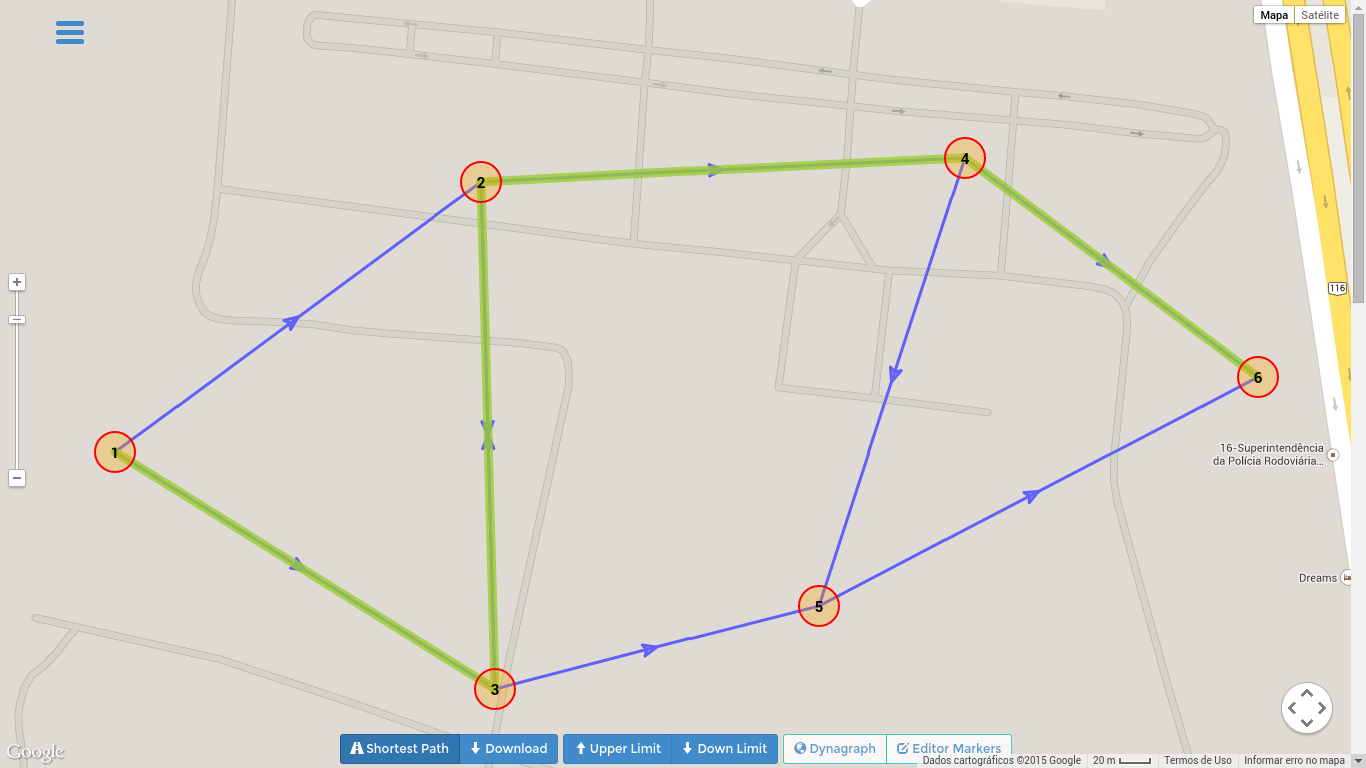
\includegraphics[width=.90\textwidth]{chapters/fig/validacao/shortestpath.png}
\caption{Simulador de Caminho Mínimo - Topologia Dinâmica e Atributos Dinâmicos}
\label{fig:shortestpath}
\end{figure}
\FloatBarrier

\begin{figure}[htbp]
\centering
 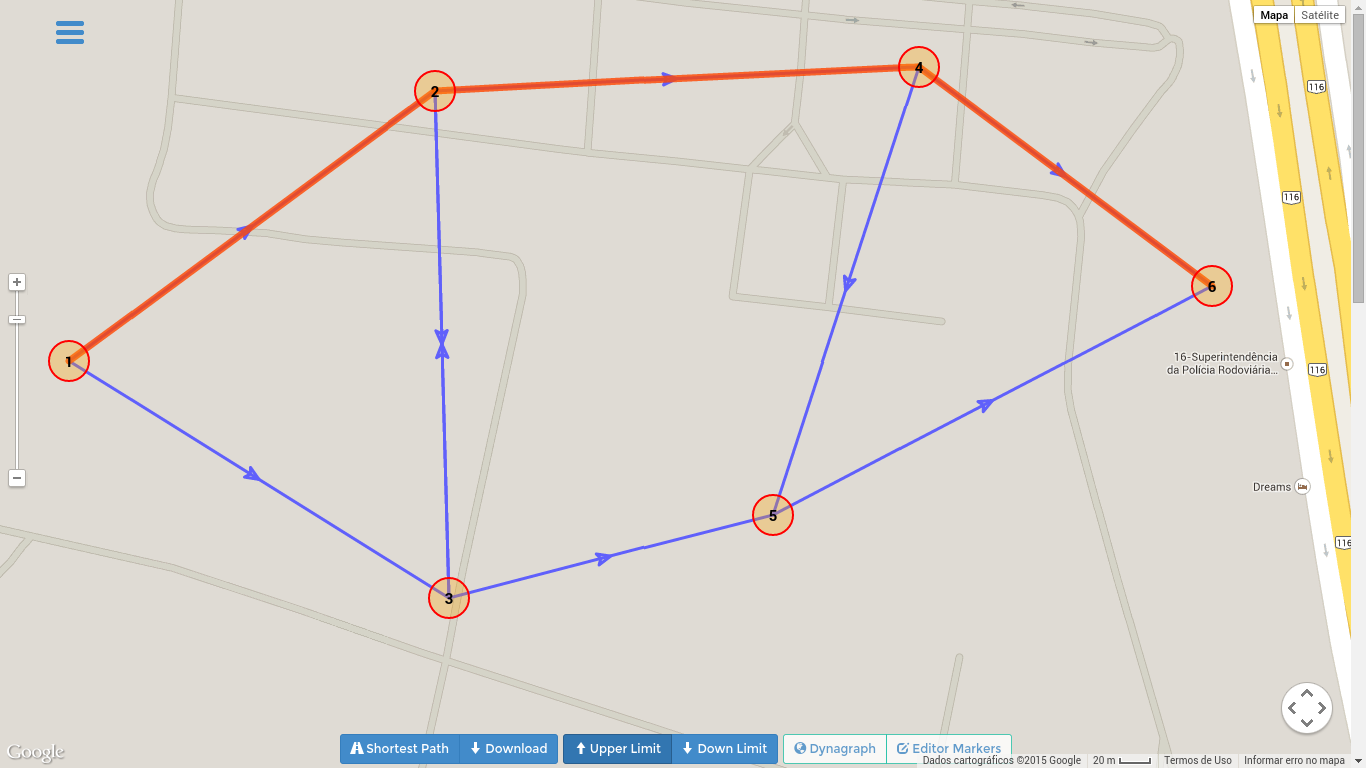
\includegraphics[width=.90\textwidth]{chapters/fig/validacao/upperlimit.png}
\caption{Simulador de Caminho Mínimo - Topologia Estática e Atributos Dinâmicos: sem permissão adiante}
\label{fig:upperlimit}
\end{figure}
\FloatBarrier

\begin{figure}[htbp]
\centering
 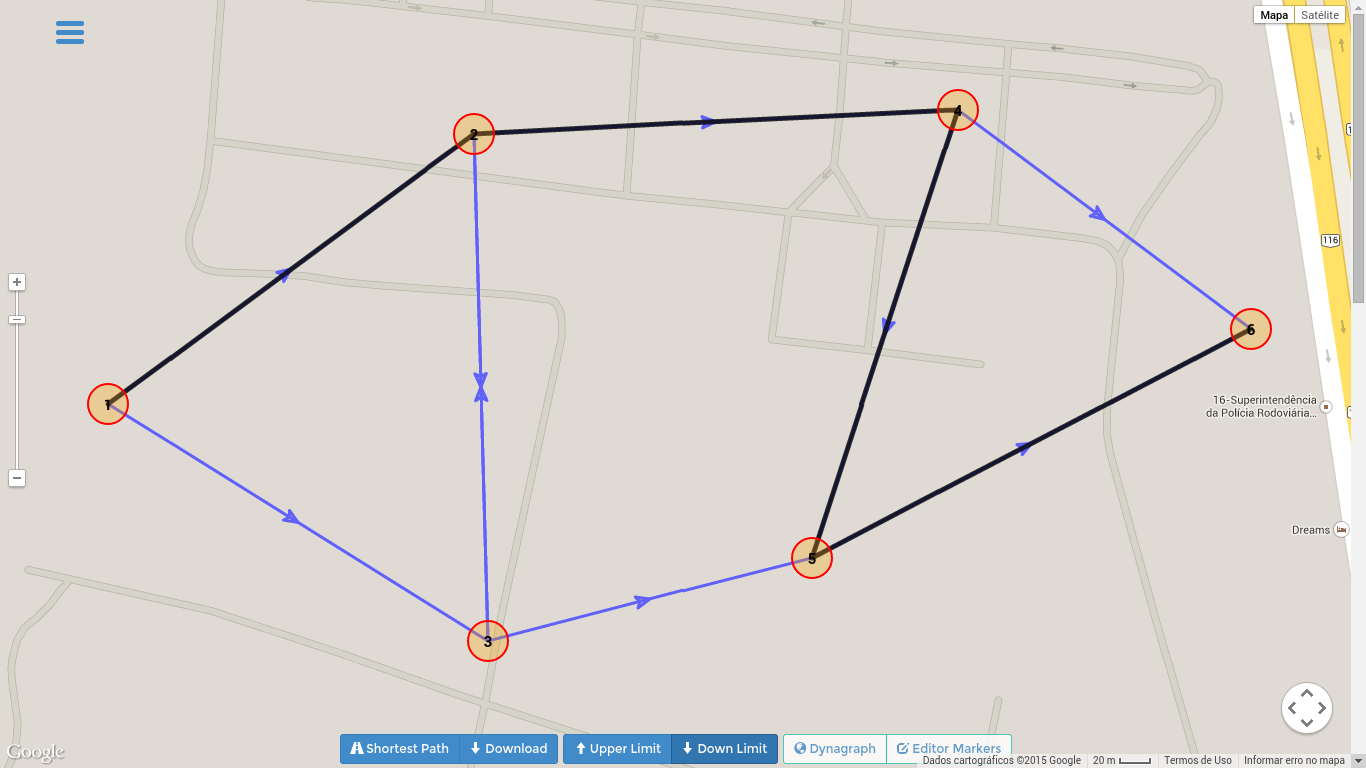
\includegraphics[width=.90\textwidth]{chapters/fig/validacao/downlimit.png}
\caption{Simulador de Caminho Mínimo - Topologia Estática e Atributos Dinâmicos: com permissão adiante}
\label{fig:downlimit}
\end{figure}
\FloatBarrier

\begin{center}
  \line(1,0){450}
\end{center}
\lstinputlisting[language=Java]{chapters/dataex1.json}
\begin{figure}[htbp]
  \begin{center}
    \line(1,0){450}
  \end{center}
  \centering
  \caption{Estrutura JSON - Exemplo 1}
  \label{fig:jsondyn}
\end{figure}
\FloatBarrier

A seguir, são apresentados os grafos gerados pela ferramenta com seus respectivos dados,
e a exibição do caminho mínimo no Dynagraph. As figuras seguem a ordem da esquerda para a direita e
de cima para baixo.

\begin{figure}[htbp]
\centering
 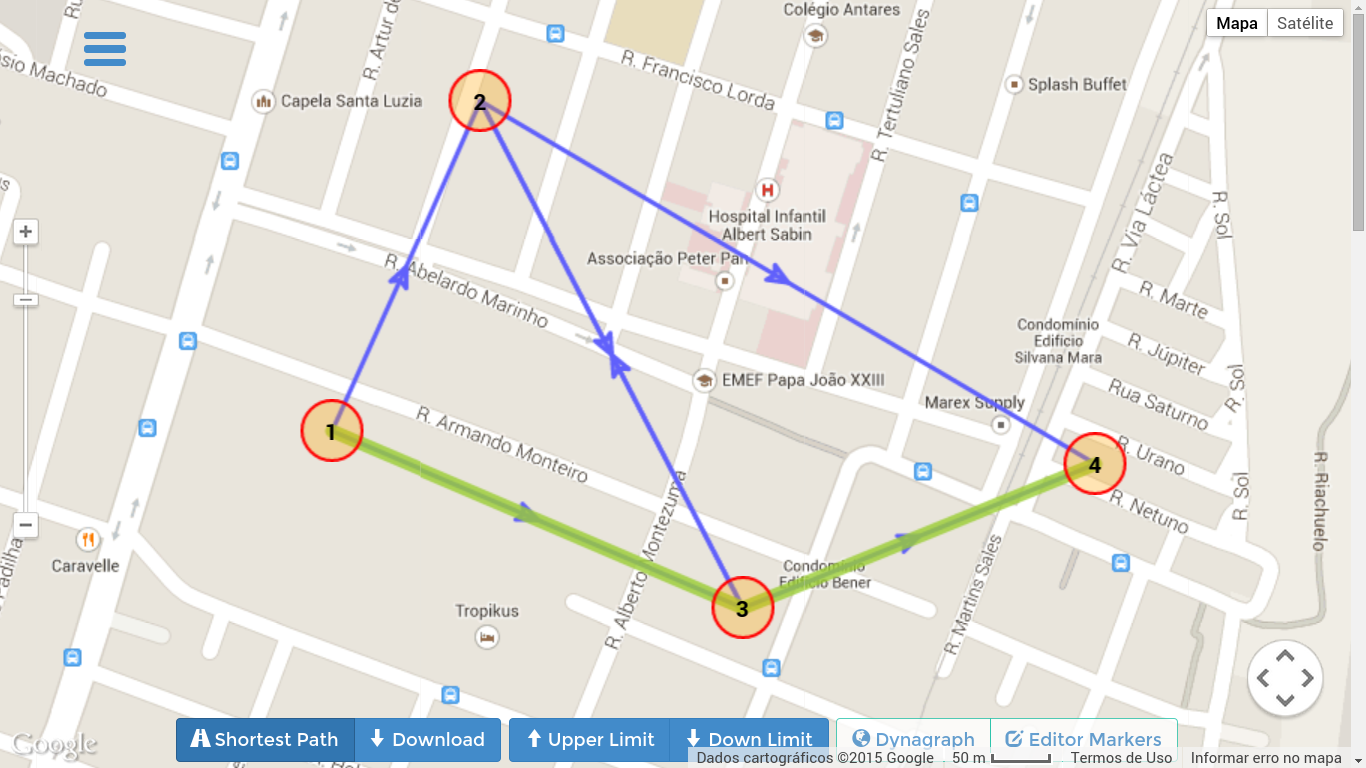
\includegraphics[width=.70\textwidth]{chapters/fig/validacao/ex1.png}
\caption{Simulador de Caminho Mínimo - Exemplo 1}
\label{fig:ex1}
\end{figure}
\FloatBarrier

\begin{figure}[htbp]
\centering
 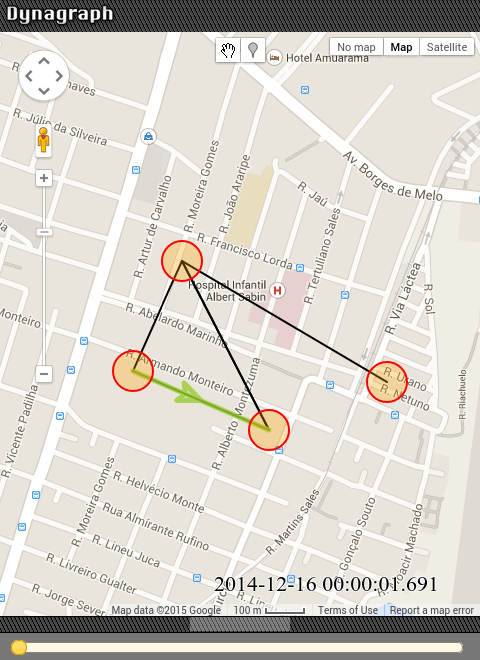
\includegraphics[width=.25\textwidth]{chapters/fig/validacao/dyn1a.png}
 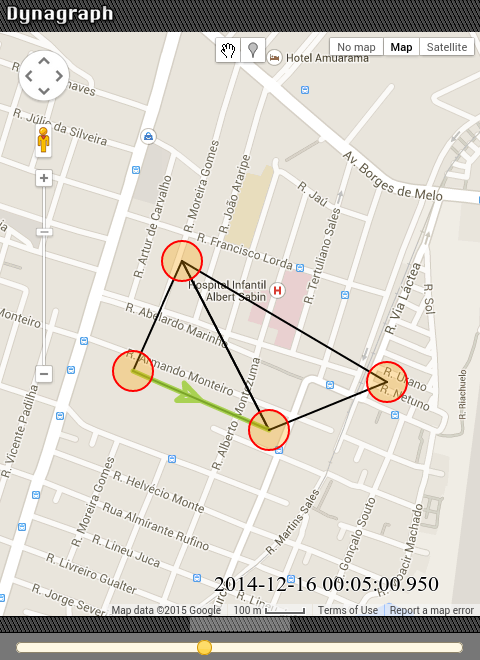
\includegraphics[width=.25\textwidth]{chapters/fig/validacao/dyn1b.png}
 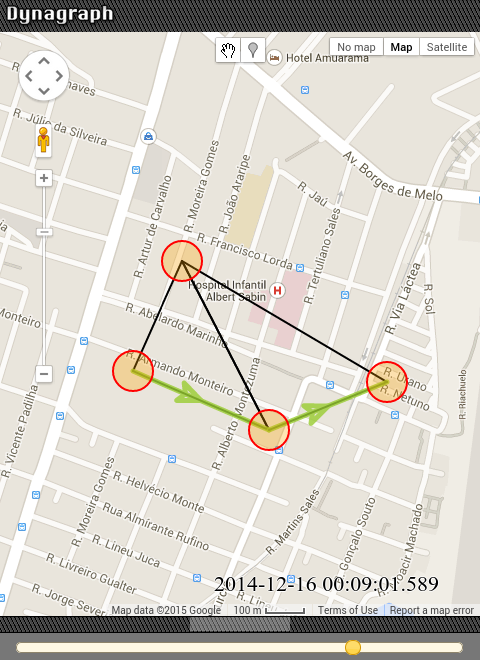
\includegraphics[width=.25\textwidth]{chapters/fig/validacao/dyn1c.png}
 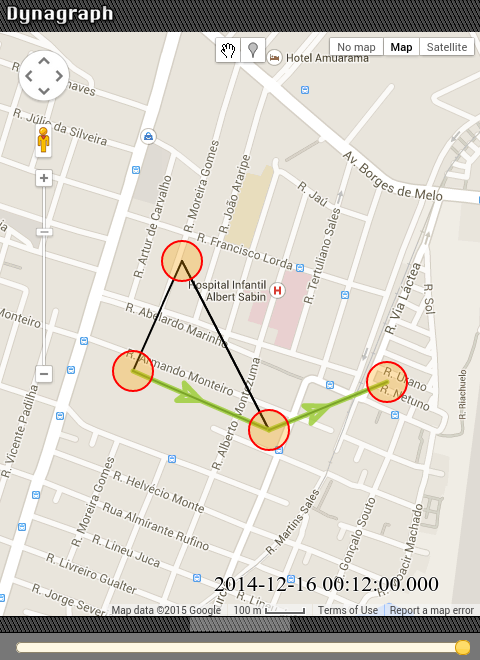
\includegraphics[width=.25\textwidth]{chapters/fig/validacao/dyn1d.png}
\caption{Caminho Mínimo no Dynagraph - Exemplo 1}
\label{fig:dyn1}
\end{figure}
\FloatBarrier

\begin{center}
  \line(1,0){450}
\end{center}
\lstinputlisting[language=Java]{chapters/fig/validacao/dyn1.json}
\begin{figure}[htbp]
  \begin{center}
    \line(1,0){450}
  \end{center}
  \centering
  \caption{Simulador de Caminho Mínimo: Estrutura JSON - Exemplo 1}
  \label{fig:jsondyn1}
\end{figure}
\FloatBarrier


\begin{figure}[htbp]
\centering
 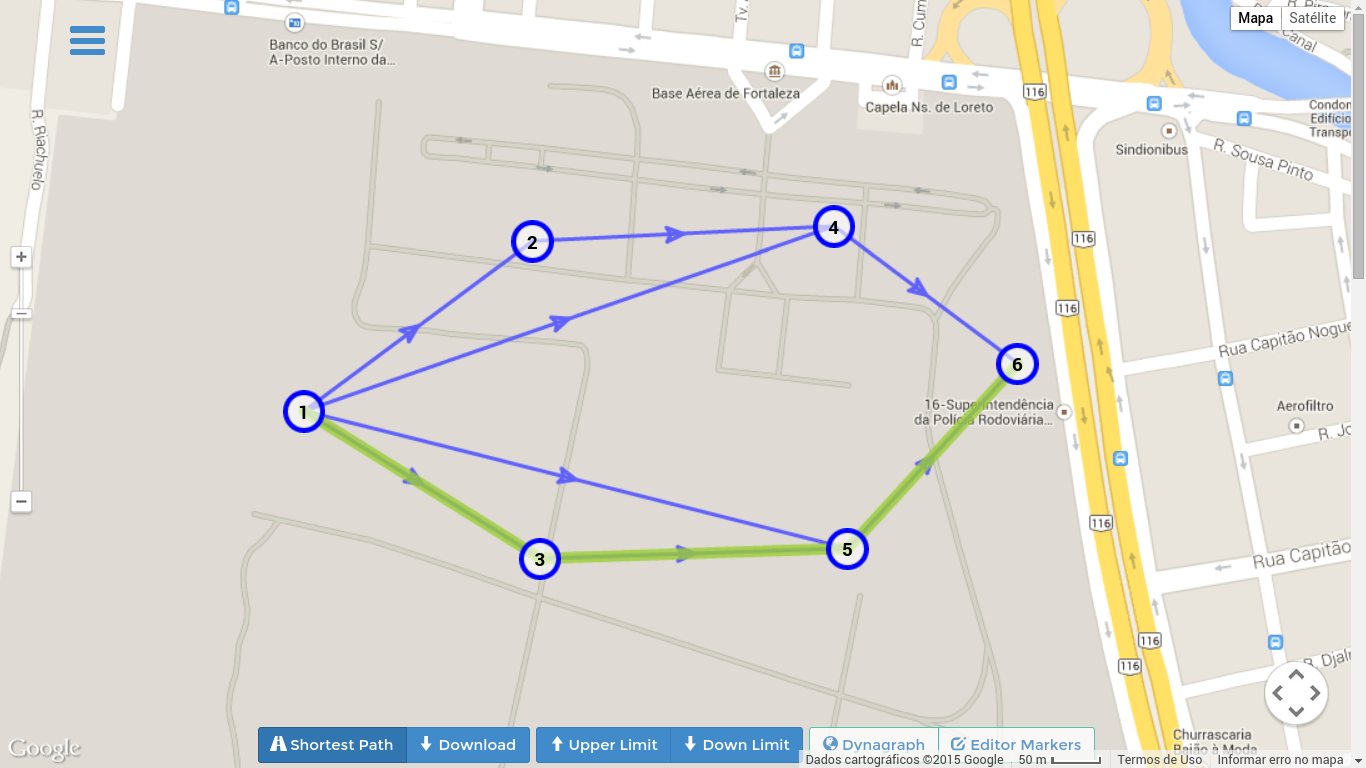
\includegraphics[width=.70\textwidth]{chapters/fig/validacao/ex2.png}
\caption{Simulador de Caminho Mínimo - Exemplo 2}
\label{fig:ex2}
\end{figure}
\FloatBarrier

\begin{figure}[htbp]
\centering
 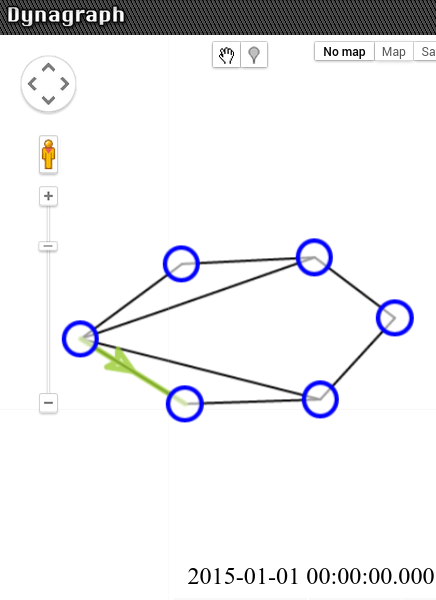
\includegraphics[width=.35\textwidth]{chapters/fig/validacao/dyn2a.png}
 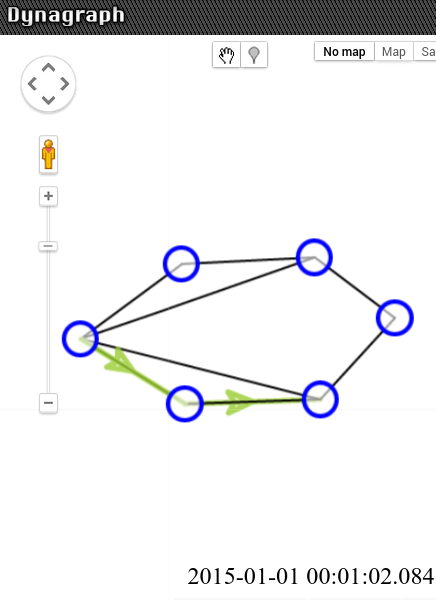
\includegraphics[width=.35\textwidth]{chapters/fig/validacao/dyn2b.png}
 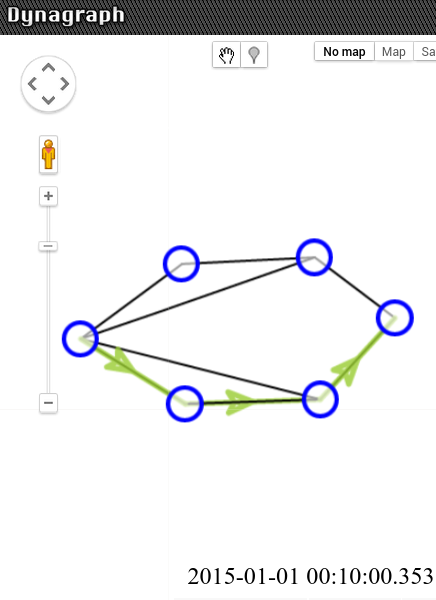
\includegraphics[width=.35\textwidth]{chapters/fig/validacao/dyn2c.png}
 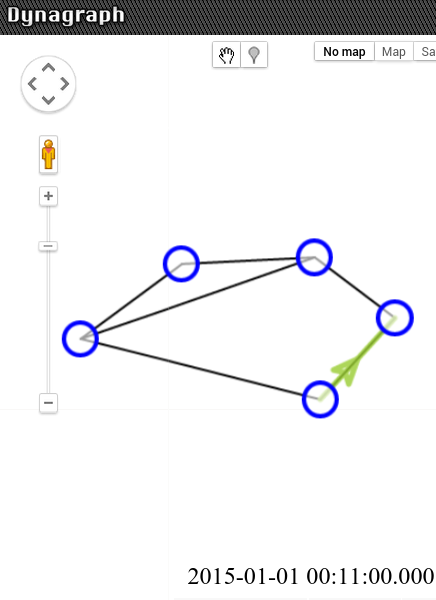
\includegraphics[width=.35\textwidth]{chapters/fig/validacao/dyn2d.png}
\caption{Caminho Mínimo no Dynagraph - Exemplo 2}
\label{fig:dyn2}
\end{figure}
\FloatBarrier

\begin{center}
  \line(1,0){450}
\end{center}
\lstinputlisting[language=Java]{chapters/fig/validacao/dyn2.json}
\begin{figure}[htbp]
  \begin{center}
    \line(1,0){450}
  \end{center}
  \centering
  \caption{Simulador de Caminho Mínimo: Estrutura JSON - Exemplo 2}
  \label{fig:jsondyn2}
\end{figure}
\FloatBarrier

A seguir, o mesmo exemplo do grafo anterior, mas com o horário de início do percurso diferente.
Percebe-se que a hora é ultrapassada, pois o percurso inicia às 23 horas e 50 minutos.
% Considerando o grafo G(N=\{P1, P2, P3, P4, P5, P6\}, A), o caminho determinado parte de P1, passa por P4 e chega em P6.

\begin{figure}[htbp]
\centering
 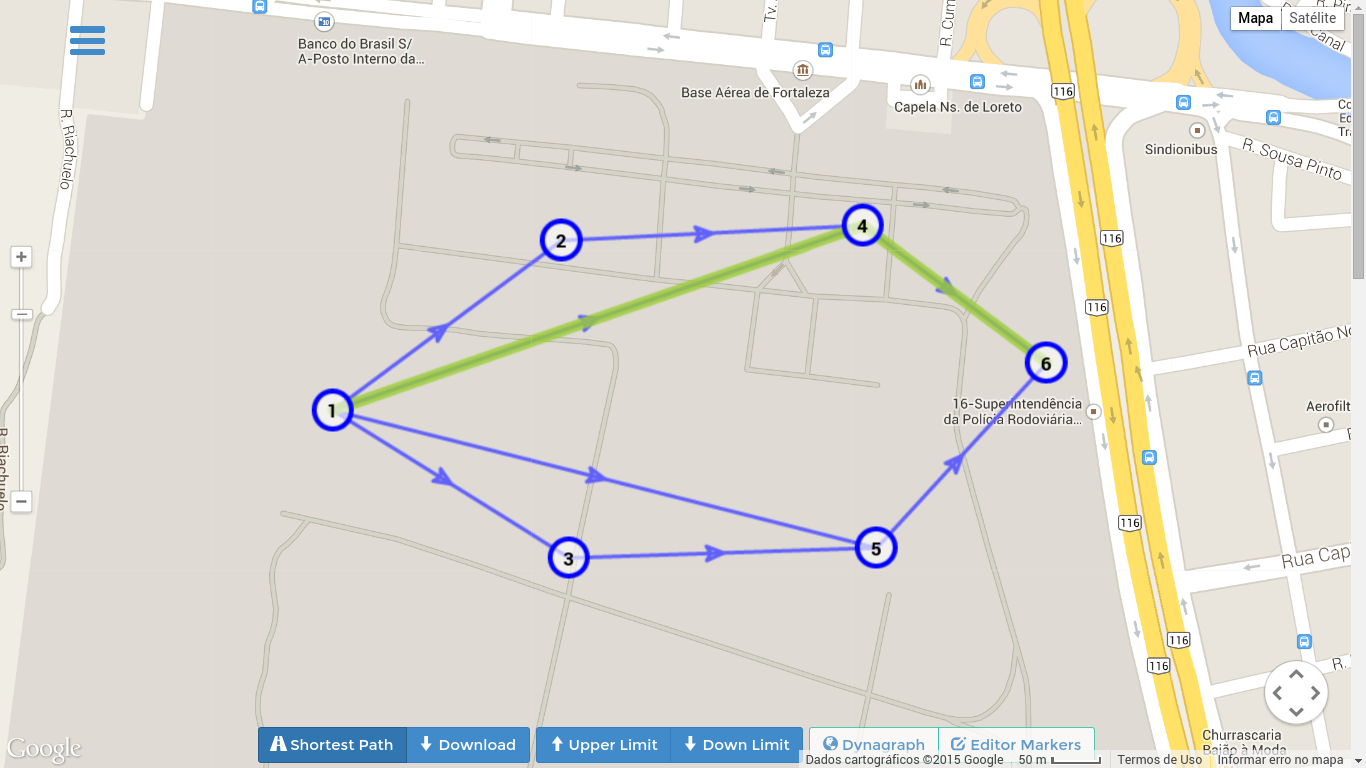
\includegraphics[width=.70\textwidth]{chapters/fig/validacao/ex3.png}
\caption{Simulador de Caminho Mínimo - Exemplo 3}
\label{fig:ex3}
\end{figure}
\FloatBarrier

\begin{figure}[htbp]
\centering
 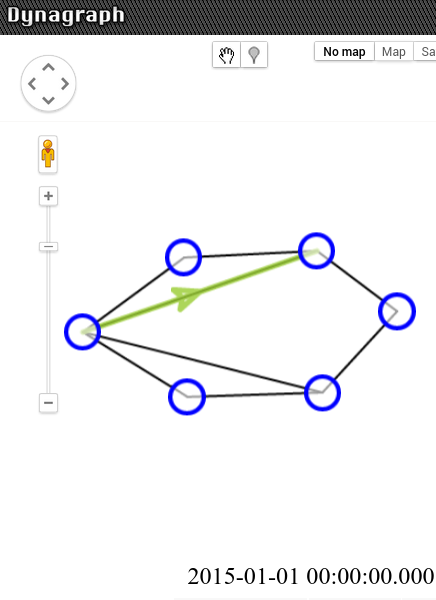
\includegraphics[width=.35\textwidth]{chapters/fig/validacao/dyn3a.png}
 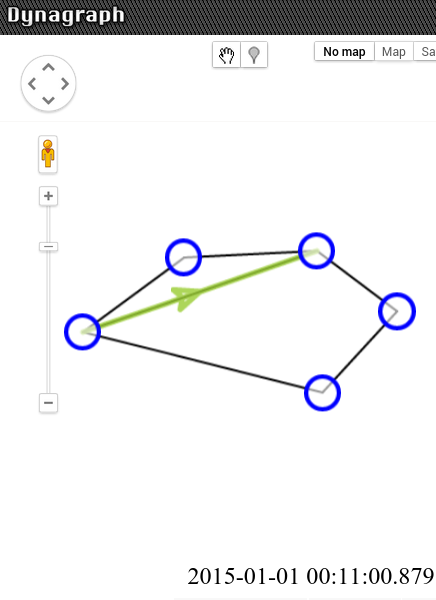
\includegraphics[width=.35\textwidth]{chapters/fig/validacao/dyn3b.png}
 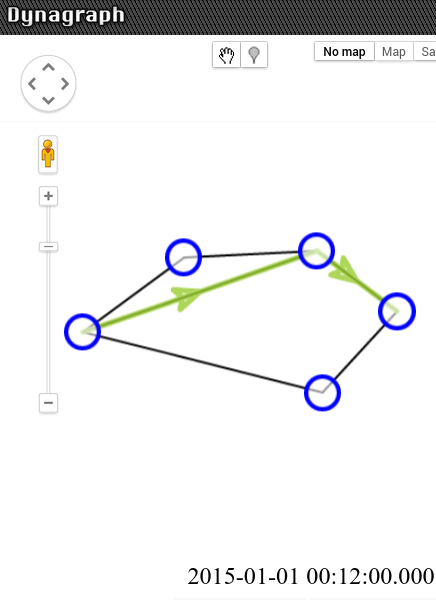
\includegraphics[width=.35\textwidth]{chapters/fig/validacao/dyn3c.png}
\caption{Caminho Mínimo no Dynagraph - Exemplo 3}
\label{fig:dyn3}
\end{figure}
\FloatBarrier

\begin{center}
  \line(1,0){450}
\end{center}
\lstinputlisting[language=Java]{chapters/fig/validacao/dyn3.json}
\begin{figure}[htbp]
  \begin{center}
    \line(1,0){450}
  \end{center}
  \centering
  \caption{Simulador de Caminho Mínimo: Estrutura JSON - Exemplo 3}
  \label{fig:jsondyn3}
\end{figure}
\FloatBarrier

Logo abaixo, um exemplo usando o mesmo vetor de custo do exemplo 3.

\begin{figure}[htbp]
\centering
 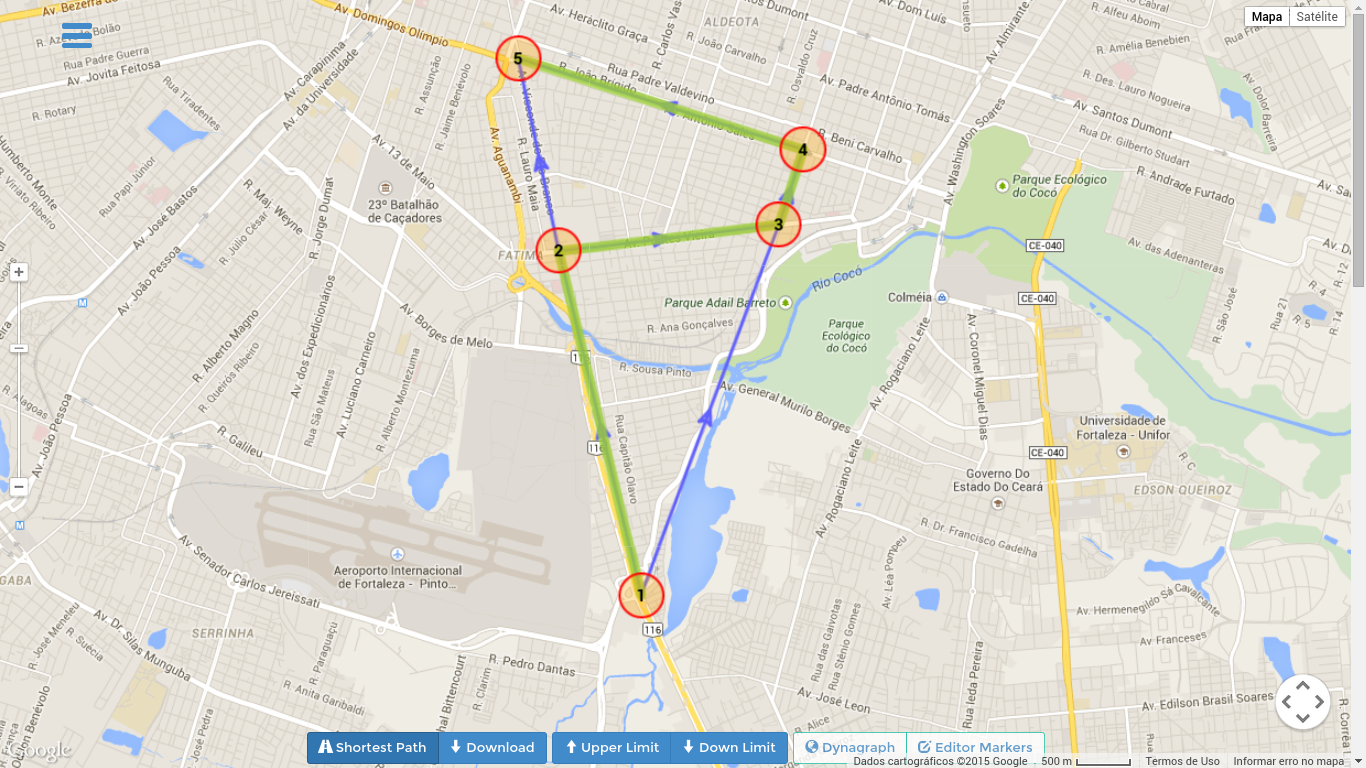
\includegraphics[width=.70\textwidth]{chapters/fig/validacao/ex4.png}
\caption{Simulador de Caminho Mínimo - Exemplo 4}
\label{fig:ex4}
\end{figure}
\FloatBarrier

\begin{figure}[htbp]
\centering
 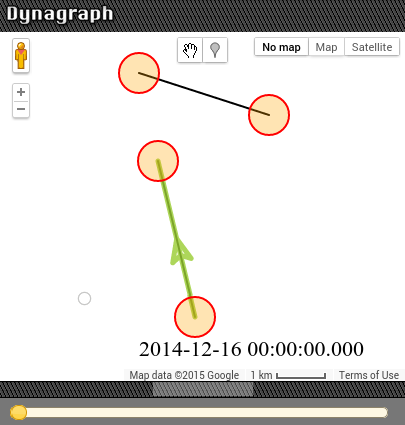
\includegraphics[width=.35\textwidth]{chapters/fig/validacao/dyn4a.png}
 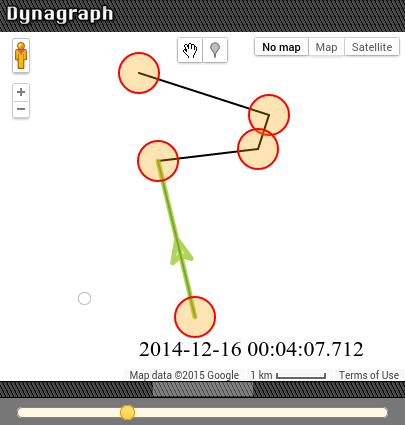
\includegraphics[width=.35\textwidth]{chapters/fig/validacao/dyn4b.png}
 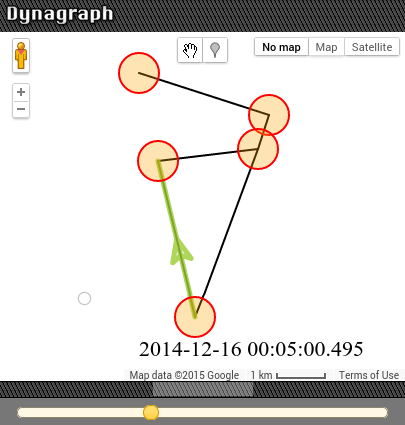
\includegraphics[width=.35\textwidth]{chapters/fig/validacao/dyn4c.png}
 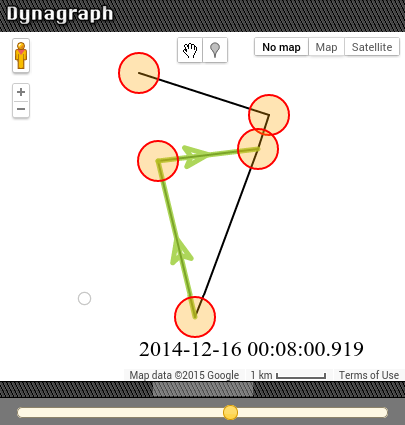
\includegraphics[width=.35\textwidth]{chapters/fig/validacao/dyn4d.png}
 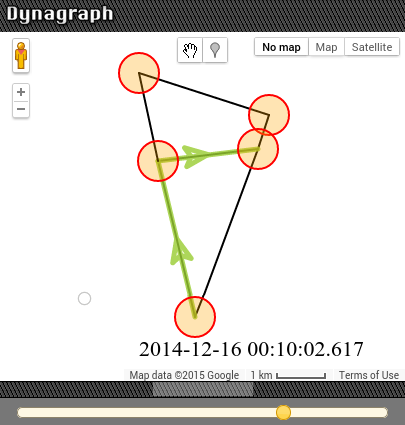
\includegraphics[width=.35\textwidth]{chapters/fig/validacao/dyn4e.png}
 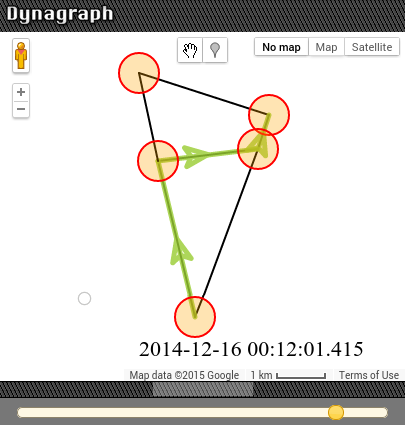
\includegraphics[width=.35\textwidth]{chapters/fig/validacao/dyn4f.png}
 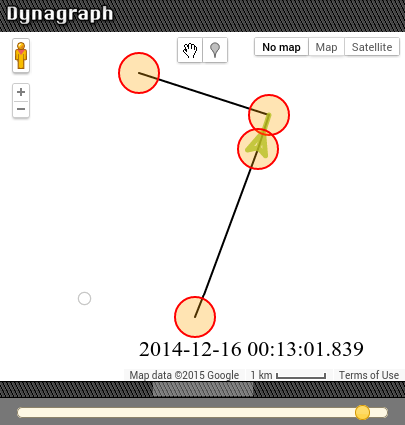
\includegraphics[width=.35\textwidth]{chapters/fig/validacao/dyn4g.png}
 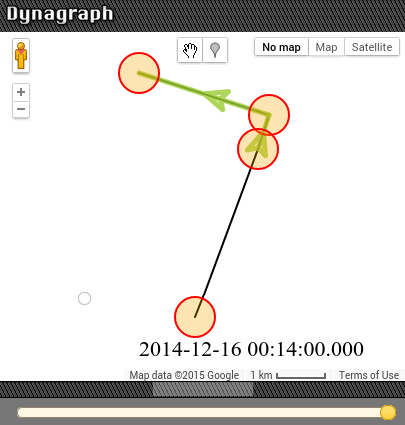
\includegraphics[width=.35\textwidth]{chapters/fig/validacao/dyn4h.png}
\caption{Caminho Mínimo no Dynagraph - Exemplo 4}
\label{fig:dyn4}
\end{figure}
\FloatBarrier

\begin{center}
  \line(1,0){450}
\end{center}
\lstinputlisting[language=Java]{chapters/fig/validacao/dyn4.json}
\begin{figure}[htbp]
  \begin{center}
    \line(1,0){450}
  \end{center}
  \centering
  \caption{Simulador de Caminho Mínimo: Estrutura JSON - Exemplo 4}
  \label{fig:jsondyn4}
\end{figure}
\FloatBarrier

\begin{figure}[htbp]
\centering
 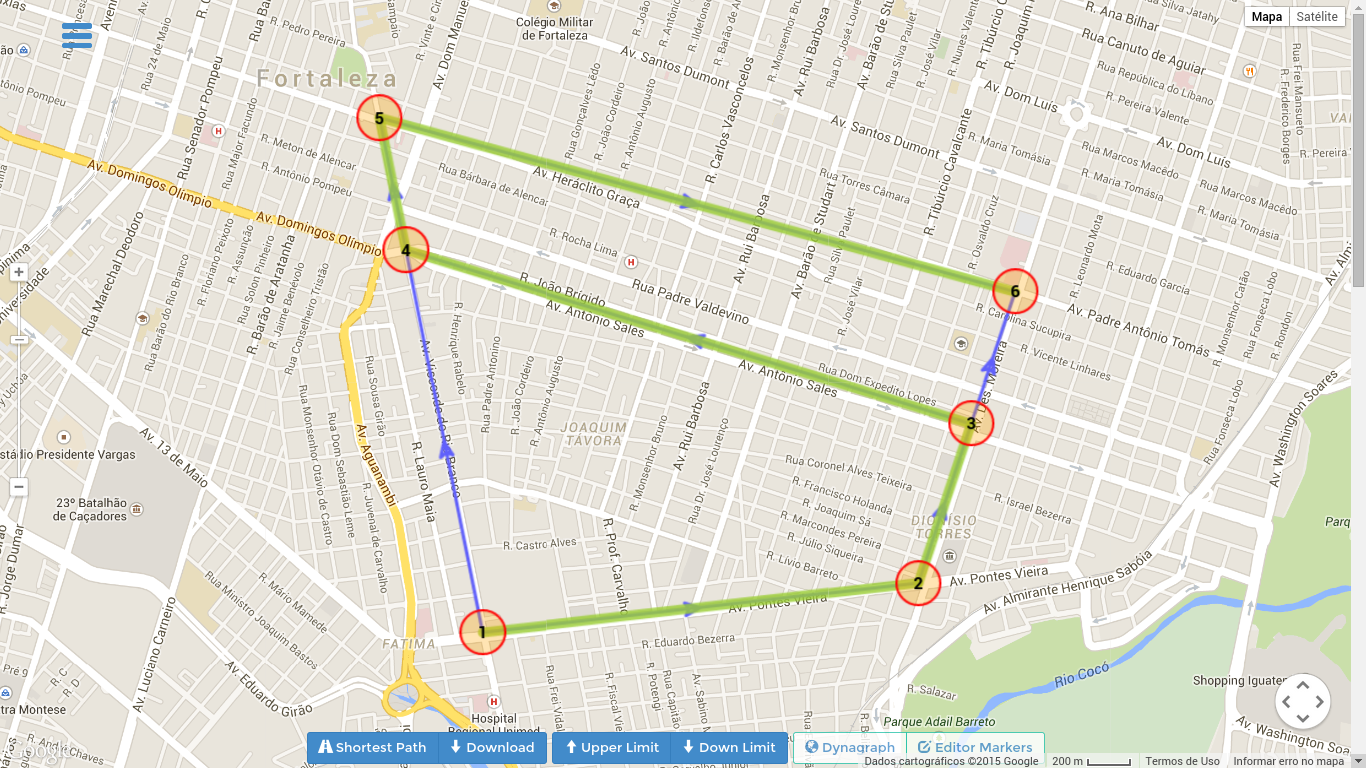
\includegraphics[width=.70\textwidth]{chapters/fig/validacao/ex5.png}
\caption{Simulador de Caminho Mínimo - Exemplo 5}
\label{fig:ex5}
\end{figure}
\FloatBarrier

\begin{figure}[htbp]
\centering
 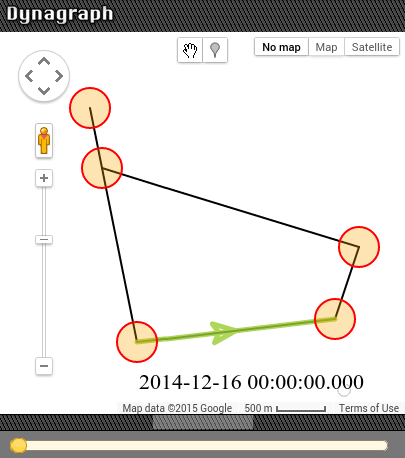
\includegraphics[width=.35\textwidth]{chapters/fig/validacao/dyn5a.png}
 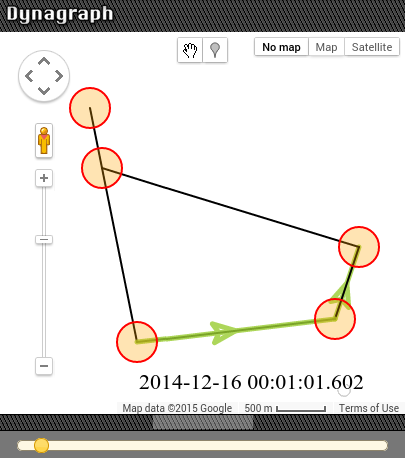
\includegraphics[width=.35\textwidth]{chapters/fig/validacao/dyn5b.png}
 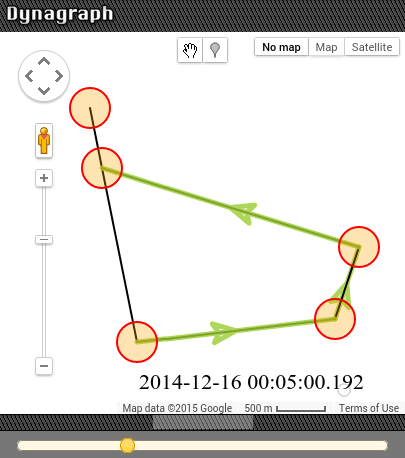
\includegraphics[width=.35\textwidth]{chapters/fig/validacao/dyn5c.png}
 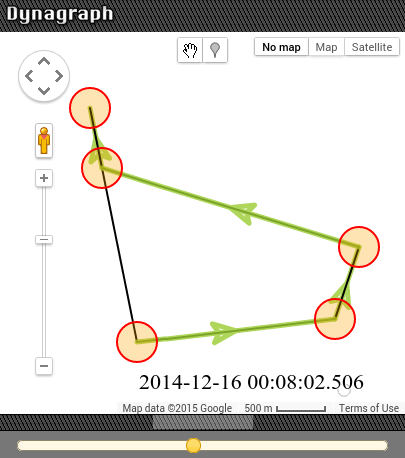
\includegraphics[width=.35\textwidth]{chapters/fig/validacao/dyn5d.png}
 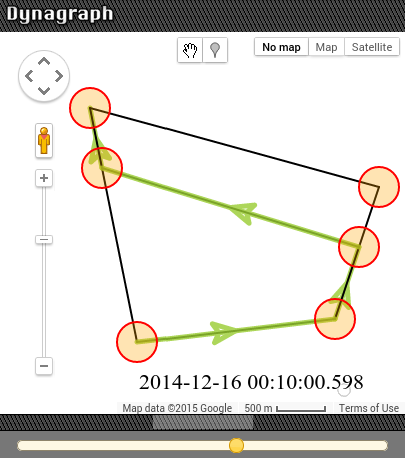
\includegraphics[width=.35\textwidth]{chapters/fig/validacao/dyn5e.png}
 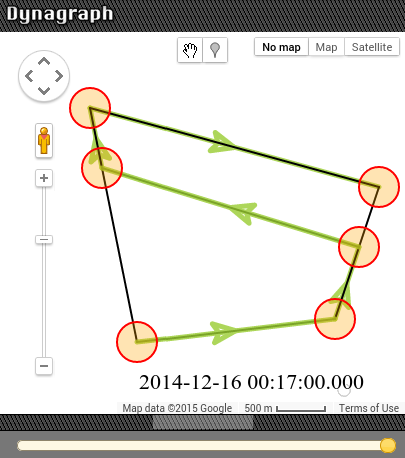
\includegraphics[width=.35\textwidth]{chapters/fig/validacao/dyn5f.png}
\caption{Caminho Mínimo no Dynagraph - Exemplo 5}
\label{fig:dyn5}
\end{figure}
\FloatBarrier

\begin{center}
  \line(1,0){450}
\end{center}
\lstinputlisting[language=Java]{chapters/fig/validacao/dyn5.json}
\begin{figure}[htbp]
  \begin{center}
    \line(1,0){450}
  \end{center}
  \centering
  \caption{Simulador de Caminho Mínimo: Estrutura JSON - Exemplo 5}
  \label{fig:jsondyn5}
\end{figure}
\FloatBarrier